\subsection{Vision Transformer}\label{s:vit}
\chapterauthor{Low Hong Sheng Jovian (2203654)}

Vision Transformers (ViT) mark a crucial adaptation of transformer architectures from textual to image analysis \cite{Khan2021Transformers}. Initially designed for natural language processing, transformers employ self-attention mechanisms which are adeptly applied to visual data in ViTs. This adaptation enables the model to dynamically prioritize different image segments according to their relevance for tasks like tumor detection in brain MRI scans.

ViTs work by breaking down an image into fixed-size patches, embedding them linearly, and treating each as a token, similar to words in text processing \cite{Wu2020Visual} (see Figure \ref{fig:vit_architecture}). Positional embeddings are added to maintain spatial relationships. These embeddings are processed through multiple transformer layers, utilizing self-attention to analyze the image holistically, enhancing the detection of complex patterns and subtle nuances indicative of tumors.

\begin{figure}[H]
  \centering
  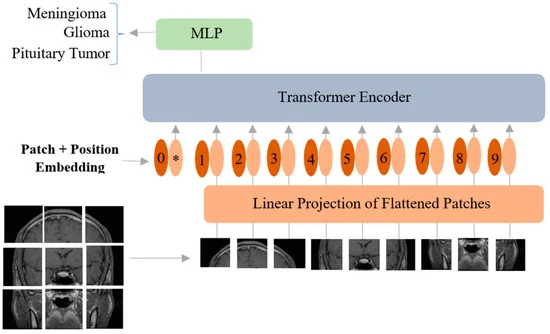
\includegraphics[width=0.45\textwidth]{vit/vit_architecture.png}
  \caption{ViT Architecture \cite{curroncol29100590}}
  \label{fig:vit_architecture}
\end{figure}

This method allows ViTs to excel in scenarios requiring deep contextual understanding and detailed image analysis. Particularly in medical imaging, ViTs are highly effective, often surpassing conventional CNNs by identifying less obvious features crucial for accurate diagnostics \cite{Matsoukas2021Is}.

Additionally, ViTs benefit from transfer learning, where models pre-trained on extensive general datasets are fine-tuned for specific medical tasks \cite{Simon2022Vision}. This not only reduces the need for large medical datasets but also speeds up the training process. Their adaptability and prowess in handling intricate image data make Vision Transformers a promising advancement in medical diagnostics, especially for improving the accuracy and reliability of brain tumor classifications.

\subsubsection{Vision Transformer Data Preprocessing}

In the initial stages of this project, several preprocessing steps were considered to optimize the performance of the ViT model for brain MRI classification. Typically, the ViT model benefits from breaking down images into smaller patches, as this allows the self-attention mechanism to effectively capture local and global features within the image. For this reason, the dataset was initially preprocessed to create patches from 224x224 pixel images. This preprocessing included resizing, cropping, normalization, and dividing the images into smaller patches.

However, during experimentation, it was observed that this approach did not yield the desired performance improvements. Specifically, the model's accuracy and ability to generalize did not improve significantly when using patched images. This was likely due to the relatively small size of the dataset, which limited the model's capacity to effectively learn from the patches. 

\begin{figure}[H]
  \centering
  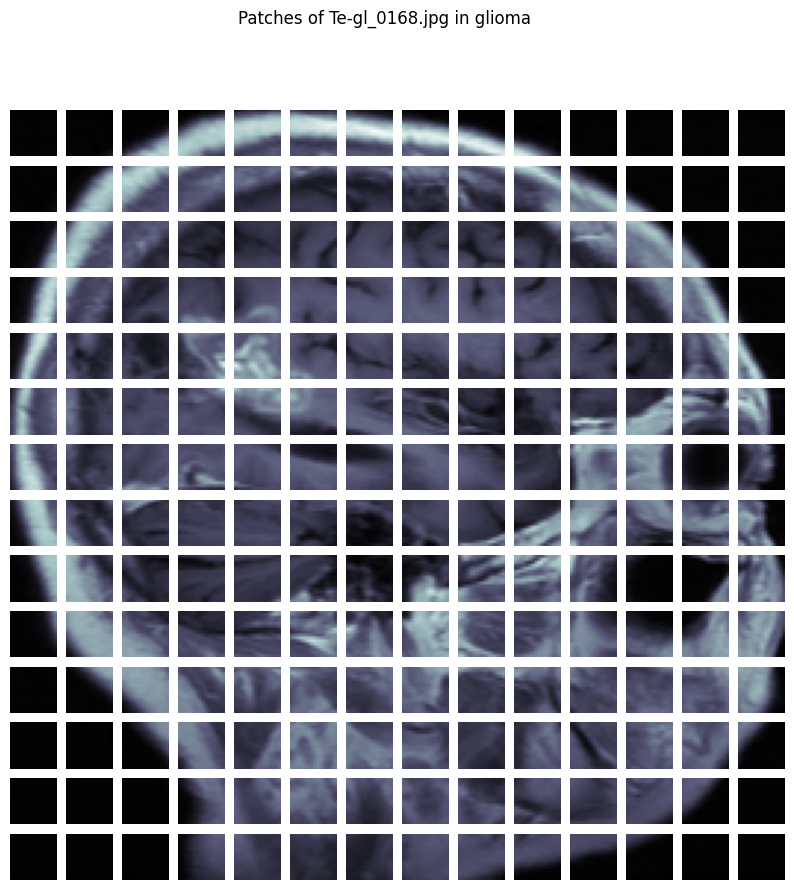
\includegraphics[width=0.45\textwidth]{vit/vit_patch.png}
  \caption{$16x16$ Patched Image}
  \label{fig:vit_patch}
\end{figure}

Furthermore, using the typical 16x16 patch size for ViT models \cite{Wang2021Not} resulted in a substantial increase in computational complexity. Each 224x224 pixel image was split into 196 patches (see Fig\ref{fig:vit_patch}), and with a total dataset size of 480 images, the resulting number of patches became unmanageable for training on available resources such as Google Colab. This immense volume of patches overwhelmed the system's memory and processing capabilities, significantly hindering the training process.

Consequently, I decided to simplify the preprocessing approach and use the pretrained ViT model directly on the original 224x224 pixel images. This decision was made to balance computational efficiency and model performance, ensuring that the training process remained feasible given the hardware constraints and dataset size.

\subsubsection{Implementation}

The proposed brain MRI classification model employs the ViT architecture, specifically the B16 variant, pretrained on the ImageNet dataset. The Vision Transformer represents a significant departure from traditional convolutional neural network models like InceptionV3, U-Net, and ResNet-50, primarily through its utilization of self-attention mechanisms. These mechanisms enable ViT to effectively capture and interpret the global context of an image, a capability that proves particularly valuable in the domain of medical image analysis, such as MRI scans. Unlike conventional models that rely on local receptive fields, ViT assesses all parts of the image in relation to one another, enhancing the detection and classification of nuanced features within complex medical images.

To specifically tailor the ViT model for brain MRI classification, several key adjustments were made. Initially, an input size of 512x512 pixels was used; however, this did not result in good performance of the model. Consequently, the input size was adjusted to 224x224 pixels with three channels, aligning with the common dimensions of medical imaging datasets. The B16 variant of the Vision Transformer was employed without its original classification head. 

\begin{figure}[H]
  \centering
  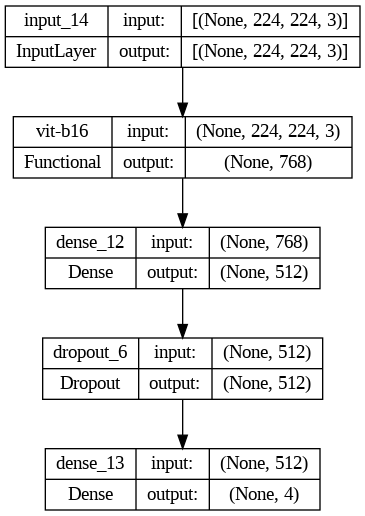
\includegraphics[width=0.45\textwidth]{vit/vit_architecture2.png}
  \caption{ViT Implemented Architecture}
  \label{fig:vit_implemented_architecture}
\end{figure}

The implemented architecture of the model is visually represented in Figure \ref{fig:vit_implemented_architecture}. It begins with an input layer that accepts images with dimensions 224x224 pixels and 3 channels (RGB). It then employs the Vision Transformer (ViT) B16 variant, which processes the input image and generates an output feature map with 768 dimensions, effectively capturing essential features while reducing dimensionality. This output is passed through a dense (fully connected) layer with 512 neurons, which helps in learning complex representations from the feature map. To mitigate overfitting, a dropout layer with a rate of approximately 32.8\% is applied next, randomly setting a fraction of input units to zero at each update during training. The final layer is another dense layer with 4 neurons, each corresponding to one of the four brain tumor classes, using a softmax activation function to convert the outputs into probabilities. This sequential architecture effectively captures and processes essential features from the input images, facilitating accurate classification of brain MRI scans into the specified tumor classes.

Typically, the output layer of ViT uses a Multi-Layer Perceptron (MLP) layer as shown in Figure \ref{fig:vit_architecture}. However, since the dataset provided is very small and ViT models are generally used for very large datasets, a softmax activation function was used instead. The softmax function is advantageous in this context because it converts the output logits into probabilities that sum to one, which is particularly useful for multi-class classification problems. This provides a clear probabilistic interpretation of the model's predictions, making it easier to identify the most likely class for each input image. The final classification layer, therefore, utilizes a softmax activation function to provide the probabilities for each class, enhancing the model's ability to make accurate predictions on diverse MRI data.

The model training and optimization involved several critical steps. The model leverages a custom Adam optimizer with a learning rate of approximately 0.0001, based on its empirical effectiveness in similar tasks involving high-dimensional image data. This choice ensures stable and gradual adjustments to the weights. The categorical cross-entropy loss function was utilized to address the multi-class nature of the classification challenge, ensuring effective discrimination between different brain tumor types. 

Training extended over 50 epochs with an early stopping mechanism that ceased training if there was no improvement in validation loss over 10 consecutive epochs. The optimal model was preserved and further assessed on a validation set, achieving a peak training accuracy of 1.000 and a validation accuracy of 0.9375 with the lowest validation loss recorded at 0.3430.


\subsubsection{Fine-Tuning}

To fine-tune the ViT model, several advanced techniques and tools were employed to optimize its performance for brain MRI classification. Initially, the batch size was systematically varied to identify the optimal setting for our specific task. After testing different batch sizes, it was determined that a batch size of 16 yielded the best performance, aligning with common practices in training Vision Transformer models \cite{Al-Hadhrami2023An}. This batch size struck a balance between computational efficiency and model accuracy, enhancing the model's ability to learn from the data without overfitting or underfitting.


In an effort to enhance the ViT model's performance for brain MRI classification, several techniques were explored. L2 regularization was applied to prevent overfitting by penalizing large weights, and some layers of the pre-trained ViT model were frozen to retain their learned features while fine-tuning the final layers. However, these approaches did not improve the model's ability to accurately classify the four classes. Consequently, they were not included in the final model's implementation.

To determine the most effective hyperparameters, the Optuna package was utilized, specifically optimizing the learning rate and dropout rate. Additionally, the training process incorporated early stopping to prevent overfitting, checkpointing to save the best model based on validation loss, and learning rate reduction on plateau to dynamically adjust the learning rate during training. These strategies collectively enhanced the model's performance and robustness, ensuring accurate classification of brain MRI scans.

Table \ref{tab:vit_finetune} summarizes the results of the fine-tuning trials, listing the validation loss for each tested dropout rate.

\begin{longtable}{|c|c|c|}
  \caption{Fine-Tuning Results for Different Dropout Rates}\label{tab:vit_finetune} \\
  \hline
  \textbf{Trial} & \textbf{Dropout Rate} & \textbf{Validation Loss} \\
  \hline
  \endfirsthead
  \caption[]{Fine-Tuning Results for Different Dropout Rates (continued)}\\
  \hline
  \textbf{Trial} & \textbf{Dropout Rate} & \textbf{Validation Loss} \\
  \hline
  \endhead
  \hline
  \endfoot
  \hline
  \endlastfoot
  Trial 1 & 0.3154 & 0.6655 \\
  \hline
  Trial 2 & 0.3336 & 0.5207 \\
  \hline
  Trial 3 & 0.3160 & 0.5524 \\
  \hline
  Trial 4 & 0.3276 & 0.3425 \\
  \hline
  Trial 5 & 0.3962 & 0.4133 \\
  \hline
  Trial 5 & 0.3962 & 0.4133 \\
  \hline
  Trial 6 & 0.3459 & 0.5437 \\
  \hline
  Trial 7 & 0.3640 & 0.6166 \\
  \hline
  Trial 8 & 0.3779 & 0.4895 \\
  \hline
  Trial 9 & 0.3845 & 0.6720 \\
  \hline
  Trial 10 & 0.3186 & 0.5634 \\
  \hline
  \end{longtable}

From this table, the optimal dropout rate was found to be trial 4 with approximately 0.3276 achieving the lowest validation loss of 0.3425. This dropout rate was selected for the final model, as it demonstrated the best performance in terms of minimizing validation loss and enhancing the model's generalization capabilities.

Through extensive experimentation using Google Colab Pro, the optimal learning rate was found to be 0.0001107117449413457, while the optimal dropout rate was determined to be 0.32755569499826637. 

% to find out where the learning rate file is and do a summary of this %

\subsubsection{Results and Evaluation}


% The confusion matrices in Figures \ref{fig:inceptionv3_cm1} and \ref{fig:inceptionv3_cm2}, provide a detailed view of the model's performance across the four brain tumor classes: meningioma, pituitary, glioma, and no tumor. The pituitary and no tumor classes exhibit slightly lower but still commendable true positive rates of 0.88, indicating strong performance across all categories. The classification report in Table \ref{tab:inceptionv3_classification_report} summarizes the precision, recall, and F1-score for each class. The model demonstrates high precision and recall across all classes, with a notable F1-score of 0.96 for the meningioma class. The overall micro, macro, and weighted averages for precision, recall, and F1-score all stand at 0.93, reflecting consistent and reliable performance.

% The ROC curve in Figure \ref{fig:inceptionv3_roc} displays the true positive rate against the false positive rate for each class. The areas under the curve (AUC) for pituitary and no tumor classes are both perfect at 1.00, while meningioma and glioma classes show AUCs of 0.97 and 0.99, respectively, indicating excellent discriminative ability of the model.

% The learning curve in Figure \ref{fig:inceptionv3_learning_curve} illustrates the model's accuracy and loss over 100 epochs. The convergence of training and validation accuracy, alongside the decreasing trend in loss values, indicates effective learning without significant overfitting.

% Table \ref{tab:inceptionv3_additional_metrics} highlights the Dice Similarity Coefficient (DSC), sensitivity, specificity, and accuracy of the model. The DSC of 0.9272 indicates a high overlap between the predicted and actual tumor regions. Sensitivity and accuracy, both at 0.9271, demonstrate the model's ability to correctly identify true positives, while the specificity of 0.9757 shows its effectiveness in correctly identifying true negatives.

\subsubsection{K-Folds Cross-Validation}

% K-Folds cross-validation was performed to evaluate the model's performance across different subsets of the dataset. The model achieved an average validation accuracy of 0.9711 and an average validation loss of 0.2188 across five folds. The model was trained for 90 epochs with a batch size of 10 for each fold. The results demonstrate the model's consistency and robustness in classifying brain tumor images.

% Results from K-Folds cross-validation are summarized in Figure \ref{f:inceptionv3_kfolds}, illustrating the validation accuracy and loss for each fold. The consistent performance across all folds, with minimal variance in accuracy and loss values, further validates the model's reliability and effectiveness in brain tumor segmentation tasks.

% Validation Accuracy: 0.9711 ± 0.0218
% Validation Loss: 0.2188 ± 0.0586
% k = 5
% epochs = 90 
% batch_size = 10


\subsubsection{Conclusion}


